\setcounter{page}{1}
\chapter{Introduction}

As the title of this thesis suggests its background is twofold. On one hand it is founded on the theory of diffusion controlled reaction rates, on the other hand it is based on transition rate theory over fluctuating barriers. \\
\section{Historic Background}
Diffusion controlled reaction rates have been studied in physics, chemistry and biology since the early 19th century. All latter inquiries on the topic are founded on the pioneering work of Marian von Smoluchowski from 1916 and 1916 who held a series of talks \cite{Smoluchowski1916} describing the motion of Brownian particles in solution and used it to describe the coagulation of gold particles \cite{Smoluchowski1917a}. Thereby he obtain the famous Smoluchowski reaction rate of ideal Brownian particles being absorbed in a spherical sink:\\
\begin{equation}
    K_S = 4 \pi D R_s \rho_0 \nonumber
    \label{Ksintro}
\end{equation}
where $D$ is the bulk diffusion constant and $\rho_0$ the bulk density of the particles and $R_s$ is the radius of the sink.\\
Later in the 1940s Debye \cite{Debye1942} extended this basic model to include inter particle interactions when he investigated the rate for diffusion limited reactions between charged particles in solution. Thereby he obtained the so called Smoluchowski Debye reaction rate:
\begin{equation}
    K_D = \rho_0\left\{\int_{R_s}^{\infty} \frac{\exp \left[ \frac{U(r')}{K_B T}\right]}{4 \pi D(r') r'^2} \rm d r' \right\}^{-1} \nonumber
    \label{Kdintro}
\end{equation}
where $D(r)$ is the spatially dependent diffusion profile, $U(r)$ is the interaction potential, $\rho_0$ is the bulk density of the particles and $R_s$ is the radius of the sink. \\
In the 1880s Szabo et. al. \cite{Szabo1982} further extended the concept to describe gating mechanisms. Therefore, the sink was no longer considered to be ideal but was taken to fluctuate between different states of surface reactivity. \\

The subject of transition rate theory has been studied empirically even since the mid 18th century by Van't Hoff \cite{hoff1884} and Arrhenius \cite{arrhenius1889} but not before 1940 it became a thorough theoretical foundation when Kramers published his celebrated paper on ``Brownian Motion in a Field of Force and the Diffusion Model of Chemical Reactions'' \cite{Kramers1940}.
He described the escape from a metastable state as a noise assisted reaction and derived the well known Kramers reaction rate.\\
Building up on Kramers results Doering and Gadoua \cite{Doering1992} were the first ones to investigate the case when the potential defining the metastable state in an escape problem is not constant but subject to fluctuations. They discovered an effect that they called \emph{resonant activation} that describes a local minimum in mean first passage times emerging from the interplay of the timescales of barrier crossing and barrier fluctuations. \\
\section{Possible Applications}
Although it seems to be a reasonable consequence of the present state of research the problem of reaction rates over fluctuating barriers has so far not been addressed. This alone being a reason for deeper investigation there is also a number of application where reaction rates over fluctuating barriers are important:
\comment{I didn't find anything on chemo-mechanical fluctuations in hydrogels. mb. looked in the wrong journals..}
\begin{itemize}
    \item Metallic nano reactors with thermo sensitive polymer shell as studied by Shuan Wu, Joachim Dzubiella et al. \cite{Wu2012a} supposedly described by a spherical sink surrounded by a potential barrier representing the solvation properties of the polymer shell. At the critical melting temperature of the polymer it undergoes a phase transition from a hydrophilic to a hydrophobic state resulting in strong fluctuations of the solvation free energy of the substrate in the region of the shell. Therefore the substrate that has to penetrate the polymer shell has to cross a fluctuating energy barrier.
    \item In recycling processes for waste water pH controlled coagulation processes are used to create flocks of organic material that can be removed by filtration \cite{Gregor1997}. In these processes the protonation of added coagulants is discrete and therefore subject to stochastic fluctuations influencing the electrostatic interaction between coagulant particles and the organic matter that is supposed to be coagulated. 
    \item The pH controlled self assembly of i.e. spider silk proteins \cite{Askarieh2010} is supposed to be dominated by the protonation of a certain domain of the protein leading to conformational changes that favor fiber formation \cite{Gaines2010}. Again the protonation of protein cites is discrete and subject to thermal fluctuations. If self assembly of the protein is described as a random walk on an energy landscape representing the possible protein conformations \cite{Rathore2002} this energy landscape is strongly influenced by the charge conformation of the protein and therefore fluctuating due to the stochastic nature of protonation. Consequently the problem is that of a random walk on a fluctuating energy landscape with one absorbing state representing the final conformation of the protein.
\end{itemize}

\section{Research interest}
As a feasible approach to the problem this thesis will study a spherical sink that is surrounded by a step shaped potential barrier fluctuating in hight and embedded in a bath of Brownian particles as illustrated in figure \ref{introSketch}. The limits of very fast and very slow barrier fluctuations can easily be deduced in analogy to the escape problem studied by Doering and Gadoua. \par
\begin{wrapfigure}[21]{o}{0.64 \textwidth}
    \hspace{-2 cm}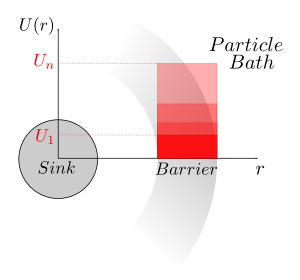
\includegraphics[width = 1.1 \textwidth]{plots/IntroSkizze.pdf}
    \caption{Sketch of system consisting of a spherical sink surrounded by a spherically symmetric step shaped barrier (indicated in \textcolor{red}{red}) embedded in a bath of Brownian particles.}
    \label{introSketch}
\end{wrapfigure}
For barrier fluctuations that are fast compared to the diffusional relaxation of the Brownian particles it can be assumed that the particles move subject to a potential of mean force, such that the rate approaches that over an average barrier. For barrier fluctuations that are very slow compared to the diffusional relaxation of the particles the rate approaches the average of the rates over the different barrier configurations. \\

If it is not possible to separate the timescales of particle diffusion and barrier fluctuations more complex behavior arises. This behavior will be the main focus of this thesis. 
Other points of interest are the dependence of effects on the spherical geometry of the system and the connection to experiment and simulations where it is common practice to reduce complex systems to only their reaction coordinates which often leads to complex diffusivity profiles and non Markovian behavior.

\section{Structure and Reading Advice}
To follow an educative approach chapter \ref{Short_Introduction_to_Stochastic_Processes} gives a short introduction to stochastic processes as far as it is helpful to supplement A) the examples from diffusion controlled reaction theory in section \ref{K_s} and \ref{The_Debye_Reaction_Rate} and B) the derivations made in section \ref{Reaction_Rates_over_Fluctuating_Barriers}. \\
Chapter \ref{Reaction_Rates_over_Fluctuating_Barriers} gives an analytical treatment of a system consisting of a spherical sink surrounded by a metastable step shaped potential barrier that is embedded by a bath of Brownian particles and derives an expression for the rate of encounters of these particles with the sink. \\
Chapter \ref{numeric_model} gives a short resume of the numerical methods in use. Chapter \ref{results} evaluates a simple example of the system described in chapter \ref{Reaction_Rates_over_Fluctuating_Barriers}. It analyzes the effects arising from coupling between diffusional relaxation and barrier fluctuations in terms of particle fluxes, gives a thorough study of all relevant parameters and finally tries to bridge the gap to experiments by interrogating on effects that arise from the reduction of the system to only the spatial coordinates through averaging over potential fluctuations. Chapter \ref{conclusion} sums up the results and gives an outlook on further work. \\

The keen reader may skip chapter \ref{Short_Introduction_to_Stochastic_Processes} and \ref{numeric_model} since they are basically a collection of relevant textbook knowledge and proceed directly with chapter \ref{Reaction_Rates_over_Fluctuating_Barriers} and \ref{results} which contain newly obtained results. 
